\PassOptionsToPackage{unicode=true}{hyperref} % options for packages loaded elsewhere
\PassOptionsToPackage{hyphens}{url}
%
\documentclass[english,man,floatsintext]{apa6}
\usepackage{lmodern}
\usepackage{amssymb,amsmath}
\usepackage{ifxetex,ifluatex}
\usepackage{fixltx2e} % provides \textsubscript
\ifnum 0\ifxetex 1\fi\ifluatex 1\fi=0 % if pdftex
  \usepackage[T1]{fontenc}
  \usepackage[utf8]{inputenc}
  \usepackage{textcomp} % provides euro and other symbols
\else % if luatex or xelatex
  \usepackage{unicode-math}
  \defaultfontfeatures{Ligatures=TeX,Scale=MatchLowercase}
\fi
% use upquote if available, for straight quotes in verbatim environments
\IfFileExists{upquote.sty}{\usepackage{upquote}}{}
% use microtype if available
\IfFileExists{microtype.sty}{%
\usepackage[]{microtype}
\UseMicrotypeSet[protrusion]{basicmath} % disable protrusion for tt fonts
}{}
\IfFileExists{parskip.sty}{%
\usepackage{parskip}
}{% else
\setlength{\parindent}{0pt}
\setlength{\parskip}{6pt plus 2pt minus 1pt}
}
\usepackage{hyperref}
\hypersetup{
            pdftitle={Computational Tools for Aural Skills Pedagogy},
            pdfkeywords={aural skills, computational musicology, survey methods, assessment},
            pdfborder={0 0 0},
            breaklinks=true}
\urlstyle{same}  % don't use monospace font for urls
\usepackage{graphicx,grffile}
\makeatletter
\def\maxwidth{\ifdim\Gin@nat@width>\linewidth\linewidth\else\Gin@nat@width\fi}
\def\maxheight{\ifdim\Gin@nat@height>\textheight\textheight\else\Gin@nat@height\fi}
\makeatother
% Scale images if necessary, so that they will not overflow the page
% margins by default, and it is still possible to overwrite the defaults
% using explicit options in \includegraphics[width, height, ...]{}
\setkeys{Gin}{width=\maxwidth,height=\maxheight,keepaspectratio}
\setlength{\emergencystretch}{3em}  % prevent overfull lines
\providecommand{\tightlist}{%
  \setlength{\itemsep}{0pt}\setlength{\parskip}{0pt}}
\setcounter{secnumdepth}{0}

% set default figure placement to htbp
\makeatletter
\def\fps@figure{htbp}
\makeatother

% Manuscript styling
\usepackage{upgreek}
\captionsetup{font=singlespacing,justification=justified}

% Table formatting
\usepackage{longtable}
\usepackage{lscape}
% \usepackage[counterclockwise]{rotating}   % Landscape page setup for large tables
\usepackage{multirow}		% Table styling
\usepackage{tabularx}		% Control Column width
\usepackage[flushleft]{threeparttable}	% Allows for three part tables with a specified notes section
\usepackage{threeparttablex}            % Lets threeparttable work with longtable

% Create new environments so endfloat can handle them
% \newenvironment{ltable}
%   {\begin{landscape}\begin{center}\begin{threeparttable}}
%   {\end{threeparttable}\end{center}\end{landscape}}
\newenvironment{lltable}{\begin{landscape}\begin{center}\begin{ThreePartTable}}{\end{ThreePartTable}\end{center}\end{landscape}}

% Enables adjusting longtable caption width to table width
% Solution found at http://golatex.de/longtable-mit-caption-so-breit-wie-die-tabelle-t15767.html
\makeatletter
\newcommand\LastLTentrywidth{1em}
\newlength\longtablewidth
\setlength{\longtablewidth}{1in}
\newcommand{\getlongtablewidth}{\begingroup \ifcsname LT@\roman{LT@tables}\endcsname \global\longtablewidth=0pt \renewcommand{\LT@entry}[2]{\global\advance\longtablewidth by ##2\relax\gdef\LastLTentrywidth{##2}}\@nameuse{LT@\roman{LT@tables}} \fi \endgroup}

% \setlength{\parindent}{0.5in}
% \setlength{\parskip}{0pt plus 0pt minus 0pt}

% \usepackage{etoolbox}
\makeatletter
\patchcmd{\HyOrg@maketitle}
  {\section{\normalfont\normalsize\abstractname}}
  {\section*{\normalfont\normalsize\abstractname}}
  {}{\typeout{Failed to patch abstract.}}
\makeatother
\shorttitle{Comp Tools}
\author{David John Baker\textsuperscript{1}}
\affiliation{
\vspace{0.5cm}
\textsuperscript{1} Louisiana State University}
\authornote{David John Baker completed this work while a Ph.D. student at Louisiana State University. He currently works for Flatiron School in London, England. 


Correspondence concerning this article should be addressed to David John Baker, 131 Finsbury Pavement. E-mail: davidjohnbaker1@gmail.com}
\keywords{aural skills, computational musicology, survey methods, assessment\newline\indent Word count: ~X}
\usepackage{lineno}

\linenumbers
\usepackage{csquotes}
\ifnum 0\ifxetex 1\fi\ifluatex 1\fi=0 % if pdftex
  \usepackage[shorthands=off,main=english]{babel}
\else
  % load polyglossia as late as possible as it *could* call bidi if RTL lang (e.g. Hebrew or Arabic)
  \usepackage{polyglossia}
  \setmainlanguage[]{english}
\fi

\title{Computational Tools for Aural Skills Pedagogy}

\date{}

\abstract{
Aural skills practitioners rely on expert intuition for choosing what melodies they should pick for melodic dictation, aural skills has no way to agree on the objective difficulty of melodies. While this lack of objectiveness does not matter for day-to-day of most instructors, relying on their expert intuitions to guide students to sucess, a lack of common language makes it difficult to perserve institutional knowledge of what students can be expected to do. In order to fill this current void, I suggest that aural skills practitioners again cross the bridge to music cognition to help with this. Specifically, I argue that by looking at work of features in computational musicology can provide an empirical, objective framework giving common language to talk about complexity of melodies. I describe how idea of features have been used in computational musicology, then demonstrate how these features map onto already held expert intutions by modeling results from a survey of 40 aural skills instructors of post-secondary education. Given the close modeling of opinion to what the features do, I conclude by showing how using these measures can begin as building block of common language to help understand what can be expected of students across all ability levels.
}

\begin{document}
\maketitle

\hypertarget{introduction}{%
\subsection{Introduction}\label{introduction}}

Which melody would be more difficult for a student to dictate, the melody from Figure 1 or Figure 2?
The melody from Figure 1 loosely follows a parallel period.
A double eighth note anacrusis begins the melody which rises and falls in a largely unsurprising fashion.
The double eight note motive reappears again half-way through the phrase.
The melody is mostly scalar, lacks any sort of syncopation, and the use of a non-diatonic F\# acts as an ornamental upper chromatic neighbor to the E that it embellishes.
Diatonic chords could be used to underpin each measure and create a stable, preditible harmonic rhythm.

\begin{figure}
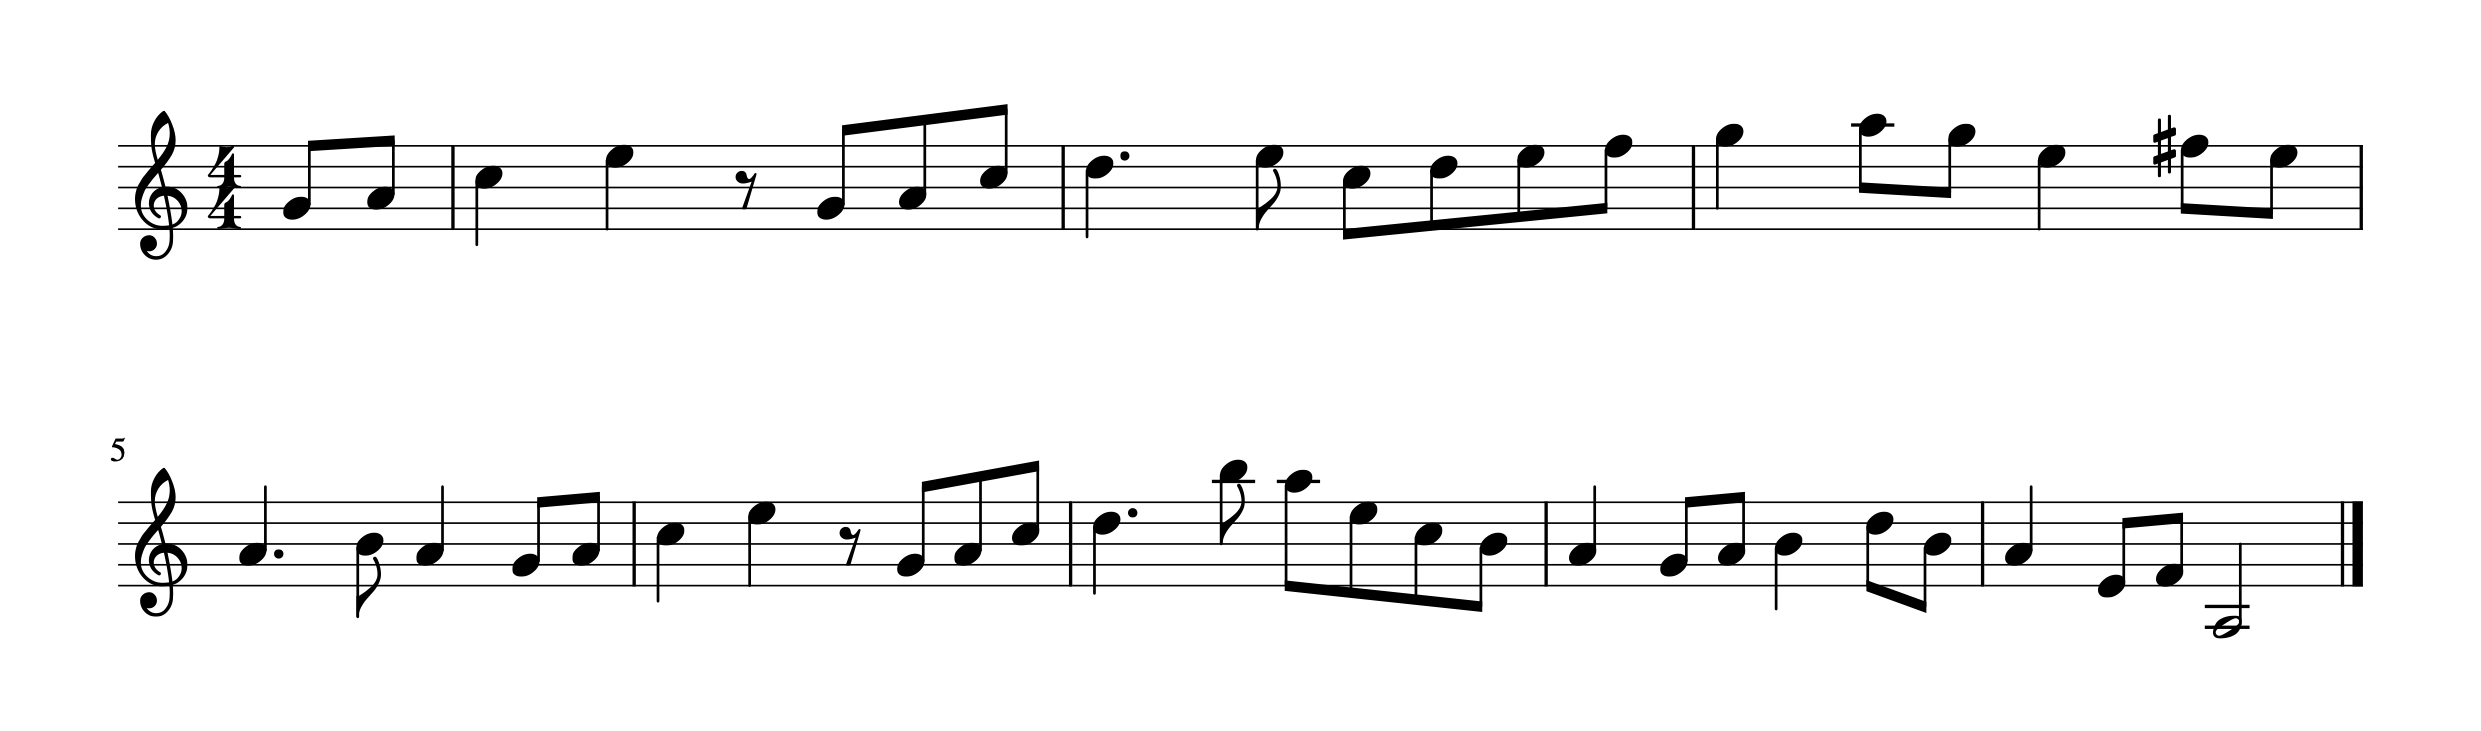
\includegraphics[width=1\linewidth]{../figures/musical_puzzles/musical_puzzle_a} \caption{A Musical Puzzle}\label{fig:puza}
\end{figure}

\begin{figure}
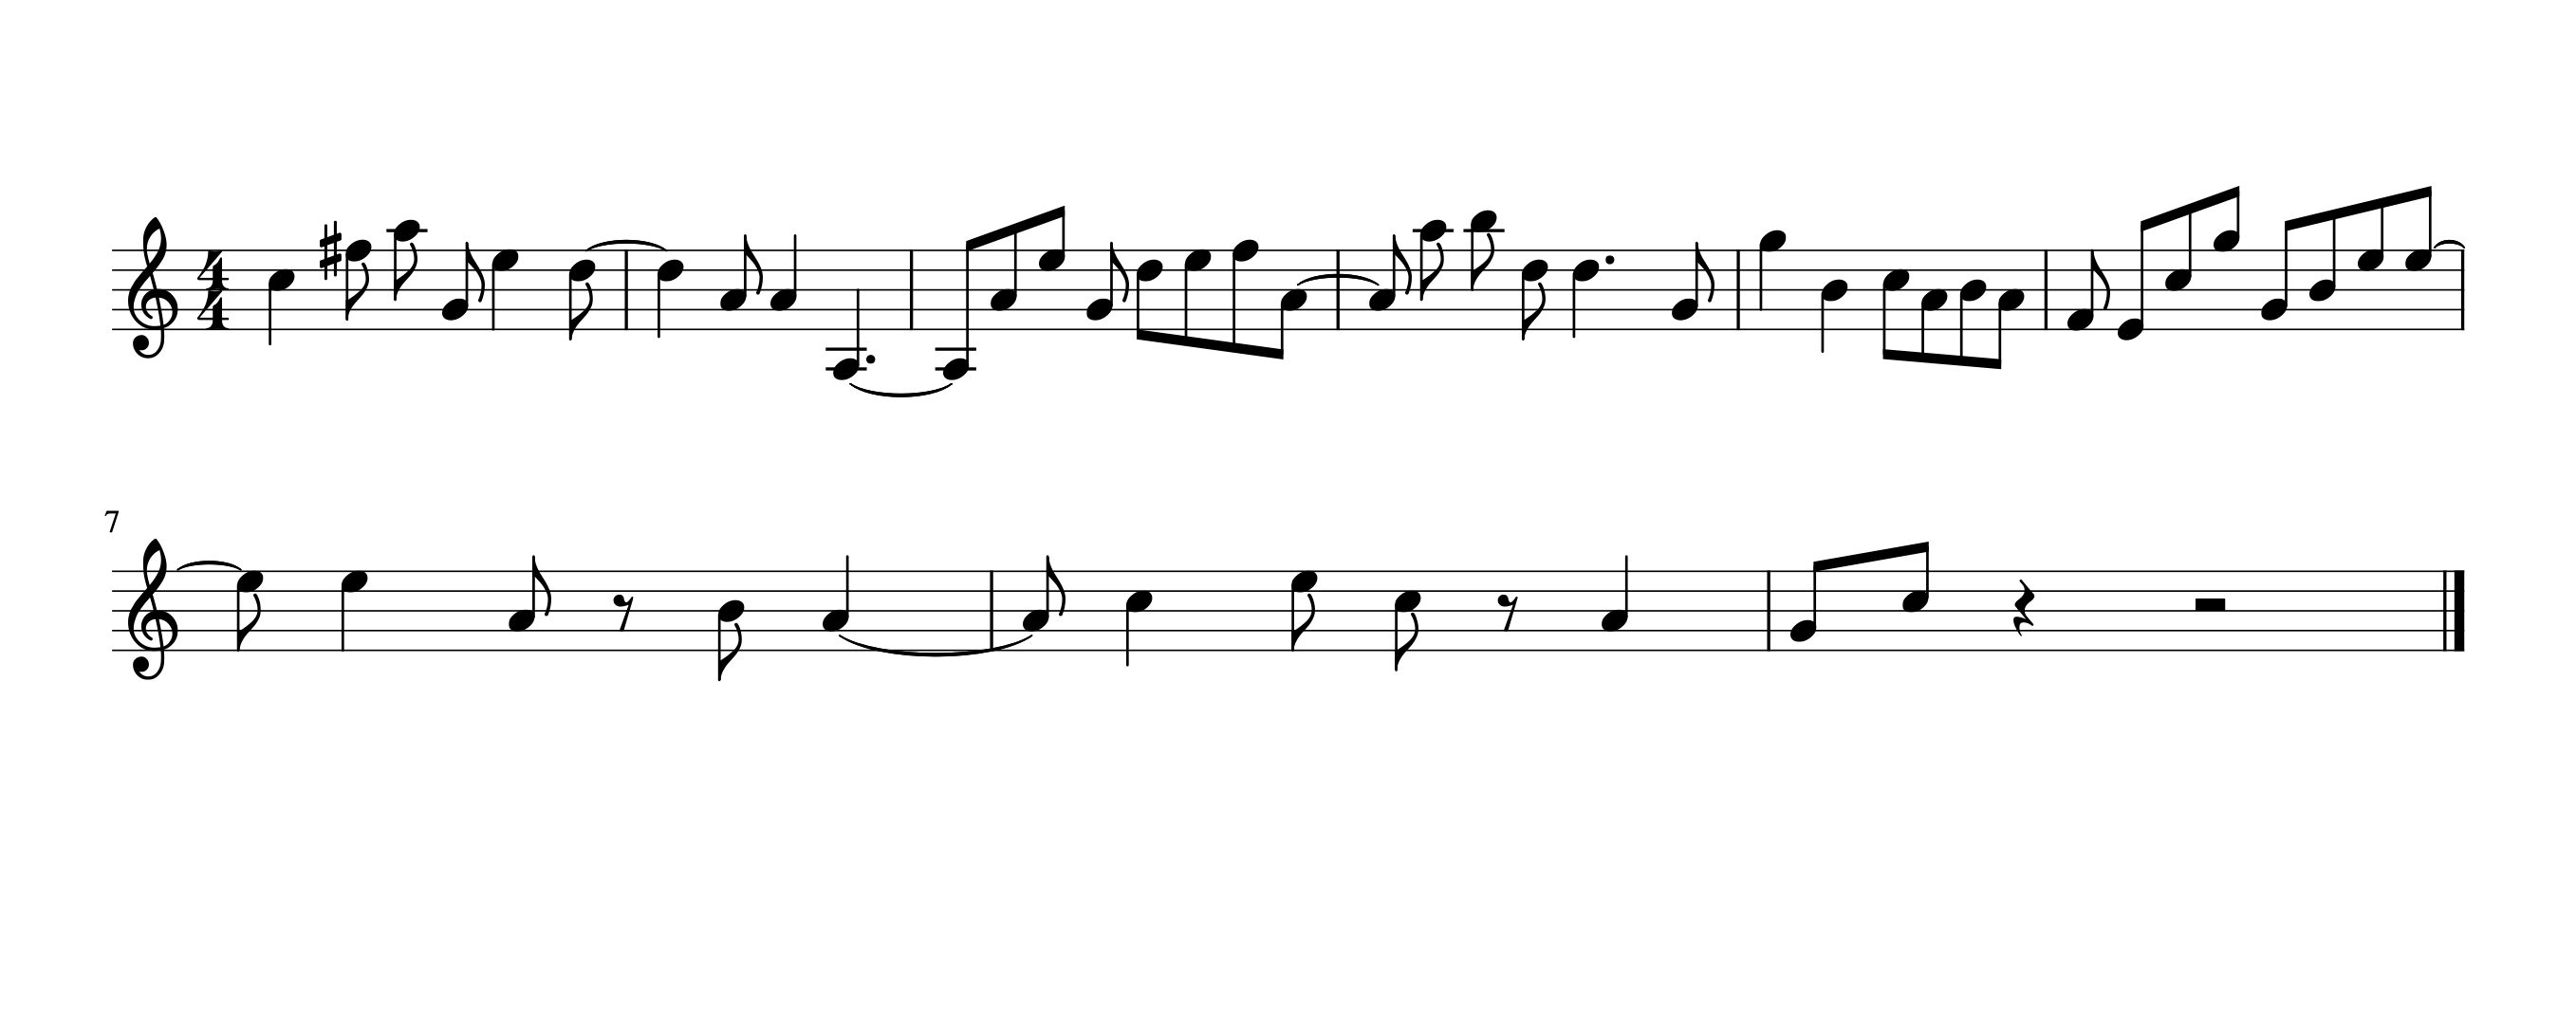
\includegraphics[width=1\linewidth]{../figures/musical_puzzles/musical_puzzle_b} \caption{B Musical Puzzle}\label{fig:puzb}
\end{figure}

In contrast, the melody from Figure 2 lacks many of the qualities listed above.
Figure 2's melody does not have a clear phrase structure, there are moments of scalar movement, but there appear to be many more leaps than anyone would want to dictate with a limited number of hearings. The syncopations both within and across the barlines obfuscate any sense of rhythmic predictibility and the introduction of the non-diatonic tone in this context-- that singular F\#-- would probably give the listener the impression this note might actually be diatonic, as it is introduced before any clear tonal center is established.

From this cursory analysis, I would assume that most aural skills students would be better at dictating the melody from Figure 1, rather than the melody from Figure 2; I think their teachers would also agree.
The answer to the opening question might have been more or less immediate for most readers of this journal and the above analysis was more just a practice in externalizing the cognition that many would intuit if forced to rank these two melodies in terms of complexity.

But what happens when this question of ranking relative difficulty were to be slightly modified?
Instead of asking a question of rank, what if it was a question of degree: how much more difficult is the melody from Figure 1 than from Figure 2?
While the answer to this question might not be immediatly useful in the day-to-day activities of aural skills instructors choosing which melodies to play to their class, being able to undestand the extent that melodies are difficult for dictation is important since it will allow instructors to be able to give their students specific, measurable, achiveable and relevant learning objectives in the case of melodic dictation.

Questions of degree are essential when considering the trajectory of a student's progress as they learn aural skills, in this case, melodic dictation.
Instructors need to know what should a student reasonably be expected to do at specific points in their of aural skills pedagogy to benchmark their progress?
Of course this answer will vary widely from institution to institution, as not all schools can or should adopt a universal standard, but a current lack of metric to describe difficulty beyond the analytical language makes it near impossible to compare between institutions and build on the field of aural skills pedagogy's collective knowledge of what constitutes a difficult melodic dictation.

Returning to the question of the extent that the melody from Figure 2 is more difficult to dictate than the melody from Figure 1, it might be possible to take an empirical stance to this question.
It could be possible to have a group of students dictate both, score them, and then make some sort of ratio comparison.
Maybe this same group of students could dictate many different melodies and the scores from each could be treated as a baseline prior from which many ratios could be constructed?

The problem with this approach is that the answer yielded would be largely dependent on the conditions of the dictation: how much experience do the students have who are dictating the melody?
Who gets to decide how many times and what tempo the melody is to be played?
Authors like Karpinski CITE have posited general rules of thumb for this that depend on the number of chunks in the melody\footnote{Footnote here about his formula}, but a lack of formalization of what constitutes a chunk as well as not including a tempo parameter in these models leaves the the insturctor with the same slippery language as above.
More importantly, if using empirical obersvations from student data were to be claimed as the metric, there also becomes the problem of determining to what extent these ratios would be stable across multiple dicatations.
Any measure that incorporates some sort of measure of student ability will be confounded based on the ability of the students contributing to the measure.

This scenario of trying to decide what melodies would be suitable for students exemplifies what aural skills instructors regularly face.
Individually, instructors might it find easy to rank the relative difficulty of melodies for our classroom using our experience and intuition for our individual learning objectives.
While this works well on a per institution, per classroom, per instructor basis, this method lacks any sort of standardization and consequently makes it difficult to communicate with other educators in order to pool resources about what any students can be expected to do.
Without an objective standard for discussing the complexity of melodies, we lack the language as community for commmond denominator to talk about the degree to which we can expect of students and continually contribute to institutional knowledge.

But if not from analytic language or the results of doing melodic dictations, where can measures of difficulty come from?
As a proxy, aural skills instructors often rely on the index melody from an aural skills textbook as a proxy for difficulty.
Presumably Melody 1 from any standard aural skills text is easier to dictate than melody 100.
But this would be putting the cart before the horse.

Assuming that having a more objective way to discuss difficulty is desirable, where do we as aural skills instructors go in order to get around this problem of relativity in grading that is subjective?
At junctures such as these, we need to cross the bridge to music cognition in order to help inform pedagogical practices CITE.
In this article, I show how tools from the field of music cognition, specifically tools from computational musicology, can help in giving aural skills pedagoges a common, objective tool in help in the disucssion of what can be reasonably expected of our students and the benefits of doing so.

\hypertarget{melodic-memory}{%
\subsection{Melodic Memory}\label{melodic-memory}}

As demonstrate in the opening narrative, reaching an objective understanding of what constitutes difficulty for music, in this case melodic dicatation, is difficult.
What is considered difficult will vary from institution to institution, thus rending terminology like \enquote{novice}, \enquote{first-semester}, or \enquote{advanced} to be relatively useless.
So how do we then find a way to move forward without makign it seem like we are trying to do a universal objective?
Is it possible to have some sort of Rosetta stone to help in this dicussion in order to help preserve institutional knowledge?

As alluded to above, when faced with difficulties in breaking down complexities associate with aural skills, the field of aural skills benefits from fruitful relationship with bridge to music cognition CITE.
Specifically, the area of resarch within music cognition research that most overlaps with melodic dictation is reserach in melodic memory.

\begin{itemize}
\item
  Dissertation Research Here
\item
  History of Features Music Ed
\item
  History of Empirical Aural
\item
  History of Features FANTASTIC
\item
  Link together
\end{itemize}

Perhaps the earliest account of studying melodic memory now extends over a centry ago with the work of Ortmann (CITE) on what he referred to as melodic determiants.
A fundamental assumption of Ortmann's work was that there were specific properties of the melody that could explain the rate at which individuals were able to recall melodic material.
Ortman concluded that XYZ were what were most helpful.

Work by Ortamann has since been extended by TAYLOR and TAYLOR AND PEMBROOK who found XYZ.
Arising from work by TP, in addition to lending evidence for XYZ, is comment from them that mention collinarity of melodies as issue to deal with.
What they mean by this is ABC.

A similar line of research in this area looks at melodic memory, BUOVIRI STUFF with educational practice.
Here is where I would add all the education literature and what htye found.
Also baker and english dissertation and such.

A parallel line that also looks at melodic memory happens in cognition.
Not done in dictation like studies above, but rather simillar different here are reserachers that have tried to predict how well people remember melodies.
- HAPLERN MULLEN
- JAKUBOWSKI
- PETER
- FRONTIEERS

Also see work with IDYOM.

All of which use idea that melodic material can predict.
This is of course hard to disentangle, but unlike using analytic language and emprical scores, have the advantage of using information from just the melody itself.
This is an attempt to formalize what those properties are, really just features, still collinar, but solid here.

\hypertarget{features}{%
\subsubsection{Features}\label{features}}

\begin{itemize}
\tightlist
\item
  What are features?
\item
  Static and Dynamic
\item
  Example of Static
\item
  Good and Bad
\item
  Example of Dynamic
\item
  Good and Bad
\end{itemize}

A feature is way to summarize the contents of melody after it has been digitized into discrete tokens, bascially when you make it a bunch of notes.
Features that readers from music theory and education might be familiar with are range or the more abstract idea of global key for melody.
While something like range would be objective, can see that something like key gives room for debate.
Much of work on features is inspired by computational linguistics.
For example, also might be familiar with nPVI.
Cite paper saying its misused.
But importantly is that it gives objective measure.
As discussed in Baker, can either be static or dynamic.
Here going to talk about static, dynamic, and also mention mathmatical?

Most complete toolbox of diverse features is that of Fantastic and Daniel.
Mostly used in questions of musical memory, basically exactly what aural skilsl are interested in local period, FANTASTIC has been predictive of XYZ.
Static features are just summary of the whole melody.
Advantage of this is that have single number to describe.
For example, range is xyz.
Also sometthing like interval entropy, which here is layman term, and is predictive of xy`.
These features have been shown to predict in THESE EXPERIMENTS.
This gives objective measure.

Negative sides of this is that does not match with phenomonlgocial experience.
Assumes that melody is almost heard in suspended animation.
Make joke about key here.
Note also that here get the problem where if suspended animation, then can have situation arise in Figure 2 where two melodies can have exact same rating on some metrics that assume summary but clearly at not represented at phenomongical level.
And also some of the features like note density are going ot interact iwth tempo.
And problematically, as noted in previous literature, all features going to correlate.
Hard to change one without others.
There are some ways around this (lasso, ridge) for prediction, or could take PCA approach.

On other side of this, can also look at dynamic models.
Here each token that was summeraized gets its own value associated with it.
Clearlest example of this is work from Marcus Pearce and IDyOM model.
Def of IDyOM here.
Essentially is able to make some sort of surprise rating based on information content.
Regardless of buying metaphor of brain as computer and discussion around that, variable can be predictive without invoking any sort of casual or mechanistic claims about cognition.
For example, show what IDyOM would have put for melody A and B in Figure 2 along with table of select features here.
Advantages of this lead to thinks like FFH in DJB.
Disadvantages of this is need larger ML model to get it to run and get values and assume some sort of stochastic, not deterministic like FANTASTIC.

Regardless of static versus dynamic, the idea here is that the features will provide some sort of grounding since they computed with paper trail.
More imporantly, can now answer questions of degree that were the problem before.

So then this leads to the question, now that we have common language, does it actually map onto what intuitive experience.
These would not be helpful if they were not predictive of expert intuition.
Next thing to do here would be to see if these measures will map mathmatically onto generalised cases like comparing the difficulty of dictation between melodies in Figure 1.
Before going on, need to also note that have been saying difficulty and complexity as same thing.
Whereas complexity in this context, i define to mean just the objective number from the computational measure, difficulty is going to relate but not be complexity.
Difficulty here is going to be more empirical resulting from student performance.
And note that the difficulty is emergent empirical feature that will interact with how the melody is performed.
For example, any less complex melody would become more difficult if played at either very fast or very slow tempi.

\begin{itemize}
\tightlist
\item
  This is useful only if these objective do actually approximate what is useful to pedagogues
\end{itemize}

So how is it possible to asses if one is predictive of the other and this actually would be helpful?
Next I present a survey ran to see if there were some sort of relationships here.
In fact, aural skills pedagogues tend to agree for the most part on questions of difficulty of dictation.
To demonstrate this, I surveyed 40 aural skills pedagogues who all have taught aural skills at the post-secondary level.

In this survey, participants were asked the questions presented in Table XXX and Table XXX using a sample of 20 melodies found in the a commonly used sight-singing textbook CITE.

\hypertarget{methods}{%
\subsection{Methods}\label{methods}}

To select the melodies used in this survey, I randomly sampled 30 melodies from a corpus of melodies (N = 481) from a subset of the Fifth Edition of the Berkowitz \emph{A New Approach to Sight Singing} ({\textbf{???}}) in order to ensure a representative sampling of melodies that might be used in a pedagogical setting.
After piloting the randomly sampled melodies on a colleague, I again randomly sampled half of this sub-set and then added in five more melodies that were not in the new set from earlier sections of the book in order to be more representative of materials students might find in the first two semesters of their aural skills pedagogy.
I ran the survey from January 31st of 2019 until March 7th, 2019.
The survey comprised of two sets of questions.

Six questions asked about the teaching background of respondents and these questions can be found in Table \ref{tab:surveyQuestions1}.
These questions were followed by asking participants to make five ratings over the 20 different melodies.
The five questions can be found in \ref{tab:surveyQuestions2}.
To encourage participation, two \$30 cash prizes were offered to two participants.
The survey had questions that were specifically designed to gauge their appropriateness for use in a melodic dictation context.
Participants were recruited exclusively online, and all provided consent to partaking in the data collection as approved by the Louisiana State University Institutional Review Board.

The table below contains the questions used in the demographic questionnaire.
Examples were given following each questions and can be found on the survey link.

\begin{longtable}[t]{l}
\caption{\label{tab:surveyQuestions1}Survey Questions}\\
\toprule
Demographic Questions\\
\midrule
What is your age, in years?\\
What is your educational status?\\
How many years have you been teaching Aural Skills at the University level?\\
Which type of syllable system do you prefer to use?\\
On which instrument have you gained the most amount of professional training?\\
What is the title of the last degree you received?\\
At what institution are you currently teaching?\\
\bottomrule
\end{longtable}

The table below contains the questions regarding the ratings of the melodies.
Participants either responded using ordinal categories or moved a slider that sat atop a 100 point scale.

\begin{table}

\caption{\label{tab:surveyQuestions2}Item Questions}
\centering
\resizebox{\linewidth}{!}{
\begin{tabular}[t]{l}
\toprule
Item Questions\\
\midrule
During which semester of Aural Skills would you think it is appropriate to give this melody as a melodic dictation?\\
How many times do you think this melody should be played in a melodic dictation\\
considering the difficulty you noted in your previous question?\\
Assume a reasonable tempo choice from 70-100BPM.\\
Please rate how difficult you believe this melody to be for the average second-year  undergraduate student at your institution.\\
The far left should indicate 'Extremely Easy' and the far right should indicate 'Extremely Difficult'.\\
Please rate this melody's adherence to the melodic grammar of the Common Practice  Period.\\
The far left should indicate 'Not Well Formed' and the far right should indicate 'Very Well Formed'.\\
Is this melody familiar to you?\\
\bottomrule
\end{tabular}}
\end{table}

Of the respondents, the average amount of years teaching aural skills was 8.76 years (\(SD = 7.60, R: 21-29\)).
I plotted the breakdown of the respondent's age and educational status below in Figure XXX.
Of the 40 respondents, all reported used some sort of movable system other than 2 who used a fixed system.
The sample represented over 30 different institutions.
Overall, the sample reflects a wide range of experience of teaching aural skills.
The sample contains both younger and older individuals, as well as a range of experience.
In the Figures XXX through below, I list the 20 melodies sampled.

\begin{itemize}
\tightlist
\item
  Melody Table???
\end{itemize}

\hypertarget{spare-text}{%
\subsection{Spare Text}\label{spare-text}}

\hypertarget{agreeing-on-difficulty}{%
\subsubsection{Agreeing on Difficulty}\label{agreeing-on-difficulty}}

In order to assess the degree to which pedagogues agreed on a melody for melodic dictation, I first plotted the mean ratings for each melody across the entire sample along with their standard error of the means in Figure \ref{fig:diffplot}.
The \(x\) axis uses the rank of the melodies, not their index position in the Berkowitz textbook.
I chose to use this rank order metric as the number of a melody in a textbook is presumed to be best conceptualized as an ordinal variable.
For example, it would be correct to assume that Melody 200 is more difficult than melody 2, but not by a factor of 100.

\hypertarget{r-diffplot-echofalse-fig.capdifficulty-ratings-from-surveyfig.aligncenter-out.width100-knitrinclude_graphicsimgdifficulty_plot.png}{%
\section{\texorpdfstring{\texttt{\{r\ diffplot,\ echo=FALSE,\ fig.cap="Difficulty\ Ratings\ from\ Survey",fig.align=\textquotesingle{}center\textquotesingle{},\ out.width="100\%"\}\ \#\ knitr::include\_graphics("img/difficulty\_plot.png")\ \#}}{\{r diffplot, echo=FALSE, fig.cap="Difficulty Ratings from Survey",fig.align='center', out.width="100\%"\} \# knitr::include\_graphics("img/difficulty\_plot.png") \#}}\label{r-diffplot-echofalse-fig.capdifficulty-ratings-from-surveyfig.aligncenter-out.width100-knitrinclude_graphicsimgdifficulty_plot.png}}

From Figure \ref{fig:diffplot}, there is an increasing linear trend from ratings of melodies being less difficult to more difficult across the sample.
Using an intraclass coefficient calculation of agreement using a two-way model (both melodies and raters treated as random effects), the sample reflects an interclass correlation coefficient of .79.
According to ({\textbf{???}}), this reflects a good degree of agreement between raters.
This trend across the sample appears in the opposite direction when plotting the mean values to the fourth question in Figure \ref{fig:grammarplot} from the survey reflecting the melody's adherence to the melodic grammar of the Common Practice period.

\hypertarget{r-grammarplot-echofalse-fig.capgrammar-ratings-from-surveyfig.aligncenter-out.width100-knitrinclude_graphicsimggrammar_plot.png}{%
\section{\texorpdfstring{\texttt{\{r\ grammarplot,\ echo=FALSE,\ fig.cap="Grammar\ Ratings\ from\ Survey",fig.align=\textquotesingle{}center\textquotesingle{},\ out.width="100\%"\}\ \#\ knitr::include\_graphics("img/grammar\_plot.png")\ \#}}{\{r grammarplot, echo=FALSE, fig.cap="Grammar Ratings from Survey",fig.align='center', out.width="100\%"\} \# knitr::include\_graphics("img/grammar\_plot.png") \#}}\label{r-grammarplot-echofalse-fig.capgrammar-ratings-from-surveyfig.aligncenter-out.width100-knitrinclude_graphicsimggrammar_plot.png}}

While similar trends appear here, yet in the opposite direction as expected, there is a clear breaking of linear trend in the far right potion of the graph that shows melodies that were sampled from the chapter of the corpus that contains atonal melodies.
Using an intraclass coefficient calculation of agreement using a two-way model, with melodies and raters treated as random effects, the sample reflects an interclass coefficient of .65, which according to ({\textbf{???}}) indicates a moderate degree of agreement among raters.
This lower agreement rating is most likely due to the subjectiveness of this question.
In their free text responses, many participants expressed difficulty in surmising what this meant.

The trends from Figure \ref{fig:diffplot} and Figure \ref{fig:grammarplot} occur in the opposite direction.
As the index or rank of the melody increases, so does the difficulty for the rating as would be expected.
As the index or rank of the melody increases, its adherence to subjective ratings of melodic grammar of the Common Practice period decreases.
Taken together, I ran a correlation on every one of the twenty melodies between a single rater's judged difficulty and its judged adherence to tonal expectations of the common practice era.
The correlations for all 20 melodies are plotted here in Figure \ref{fig:gramcor}.
From this chart, we see this trend is not uniform across all melodies.

\hypertarget{r-gramcor-echofalse-fig.capcorrelation-between-difficulty-and-subjective-ratings-of-tonal-grammarfig.aligncenter-out.width100-knitrinclude_graphicsimggrammar_difficulty_correlation_plot.png}{%
\section{\texorpdfstring{\texttt{\{r\ gramcor,\ echo=FALSE,\ fig.cap="Correlation\ Between\ Difficulty\ and\ Subjective\ Ratings\ of\ Tonal\ Grammar",fig.align=\textquotesingle{}center\textquotesingle{},\ out.width="100\%"\}\ \#\ knitr::include\_graphics("img/grammar\_difficulty\_correlation\_plot.png")\ \#}}{\{r gramcor, echo=FALSE, fig.cap="Correlation Between Difficulty and Subjective Ratings of Tonal Grammar",fig.align='center', out.width="100\%"\} \# knitr::include\_graphics("img/grammar\_difficulty\_correlation\_plot.png") \#}}\label{r-gramcor-echofalse-fig.capcorrelation-between-difficulty-and-subjective-ratings-of-tonal-grammarfig.aligncenter-out.width100-knitrinclude_graphicsimggrammar_difficulty_correlation_plot.png}}

Overall, the sample exhibited an acceptable degree of inter-rater reliability as measured by the interclass correlation coefficient.
Plotting the respondent's answers across the textbook that melodies were taken from, with the book progressing from less to more difficult, it does appear that aural skills pedagogues tend to agree on how difficult a melody is when used in a dictation setting.

Central to my argument, there appears to a linear trend of difficulty across the sample based on the melodies rank in the sample.
In fact, although I presented the data above as ordinal using rank in the textbook, when I ran a mixed-effects linear regression predicting melody difficulty with both rank order as a variable as well as the actual index number of the melody from the Berkowitz, the index model significantly outperforms the rank order model.
Using the lme4 package ({\textbf{???}}), I fit two linear mixed effects models predicting difficulty of melody with subject and item both as random effects in the model, with the only difference in models being a melody rank or melody index.
When comparing models, the index model (BIC = 6706.3) provided a better fit to the data (\(\chi^2\)=5.38, \(p<.05\)) than the rank model (BIC = 6711.7).

Taken together, both anecdotal and empirical evidence for this survey suggest that aural skills pedagogues tend to agree on how difficult a melody is for use in an aural skills setting.
This sense of difficulty or complexity tracks as the book progresses, but to attribute the cause of a melody being difficult as its position in the book would be putting the cart before the horse.
Having now formally established this almost intuitive notion, the remaining portion of this chapter investigates how computationally derived tools can be used to model these commonly held intuitions.
In order to provide a sense of validity to the measure, I carry forward ratings from the survey reported and use the expert answers as the ground truth for the the resulting models.

\hypertarget{discussion}{%
\subsection{Discussion}\label{discussion}}

\begin{itemize}
\tightlist
\item
  IC as just good proxy for it all
\item
  Have shown here that tools from computational musicology provide good model for agreement
\item
  Of course not perfect and should not be imposed as global standards
\item
  But tacking down this one part will allow more context when start to talk about difficulty in the actual experience
\item
  Benefits here are that we can begin to understand the meachanisms of this
\item
  If we know it better, become better teachers
\item
  And then point of all of this is if we know btter, we help students in the long run.
\end{itemize}

\hypertarget{data-analysis}{%
\subsection{Data analysis}\label{data-analysis}}

We used R (Version 3.6.2; R Core Team, 2019) and the R-packages \emph{kableExtra} (Version 1.1.0; Zhu, 2019), \emph{magrittr} (Version 1.5; Bache \& Wickham, 2014), and \emph{papaja} (Version 0.1.0.9942; Aust \& Barth, 2020) for all our analyses.

\newpage

\hypertarget{references}{%
\section{References}\label{references}}

\begingroup
\setlength{\parindent}{-0.5in}
\setlength{\leftskip}{0.5in}

\hypertarget{refs}{}
\leavevmode\hypertarget{ref-R-papaja}{}%
Aust, F., \& Barth, M. (2020). \emph{papaja: Create APA manuscripts with R Markdown}. Retrieved from \url{https://github.com/crsh/papaja}

\leavevmode\hypertarget{ref-R-magrittr}{}%
Bache, S. M., \& Wickham, H. (2014). \emph{Magrittr: A forward-pipe operator for r}. Retrieved from \url{https://CRAN.R-project.org/package=magrittr}

\leavevmode\hypertarget{ref-R-base}{}%
R Core Team. (2019). \emph{R: A language and environment for statistical computing}. Vienna, Austria: R Foundation for Statistical Computing. Retrieved from \url{https://www.R-project.org/}

\leavevmode\hypertarget{ref-R-kableExtra}{}%
Zhu, H. (2019). \emph{KableExtra: Construct complex table with 'kable' and pipe syntax}. Retrieved from \url{https://CRAN.R-project.org/package=kableExtra}

\endgroup

\end{document}
